\documentclass[a4paper,11pt]{article}

\usepackage[frenchb]{babel}
\usepackage[utf8]{inputenc}
\usepackage{verbatim}
\usepackage{graphicx}
\usepackage{listings}
\usepackage{color}

\definecolor{dkgreen}{rgb}{0,0.6,0}
\definecolor{gray}{rgb}{0.5,0.5,0.5}
\definecolor{mauve}{rgb}{0.58,0,0.82}

\lstset{frame=tb,
  language=Java,
  aboveskip=3mm,
  belowskip=3mm,
  showstringspaces=false,
  columns=flexible,
  basicstyle={\small\ttfamily},
  numbers=none,
  numberstyle=\tiny\color{gray},
  keywordstyle=\color{blue},
  commentstyle=\color{dkgreen},
  stringstyle=\color{mauve},
  breaklines=true,
  breakatwhitespace=true,
  tabsize=3
}

\begin{document}
\title{Compte Rendu du TD numéro 7 de l'équipe Eirb'Reteau}
\date{Pour le 18 novembre 2014}
\maketitle

\begin{center}
  Coordinateur : Aurélien Nizet \\
  Tandem 1 : Pierre Gaulon, Victor Dury \\
  Tandem 2 : Lionel Adotevi, Reda Boudjeltia  \\
\end{center}
\maketitle
\section{Introduction}





\begin{figure}

    \caption{Diagramme de class A-UN}
    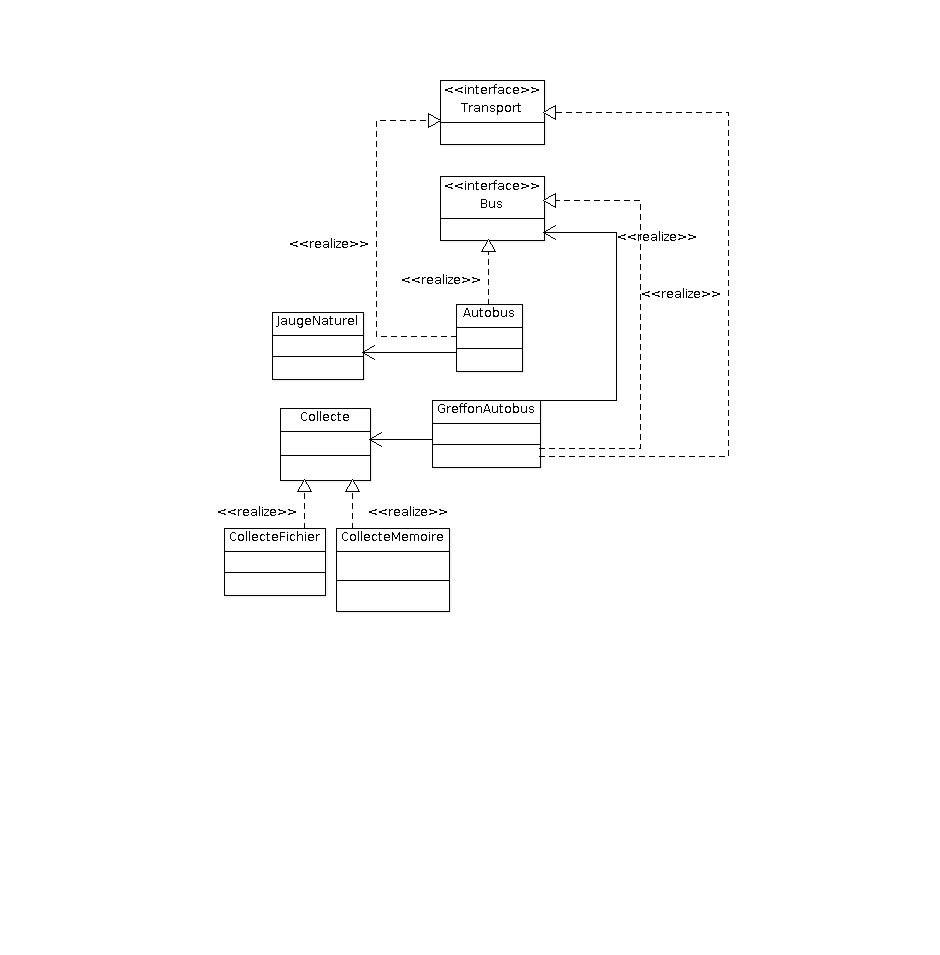
\includegraphics[scale=0.4]{a-un.png}

\end{figure}



\begin{figure}

    \caption{Diagramme de class EST-UN}
    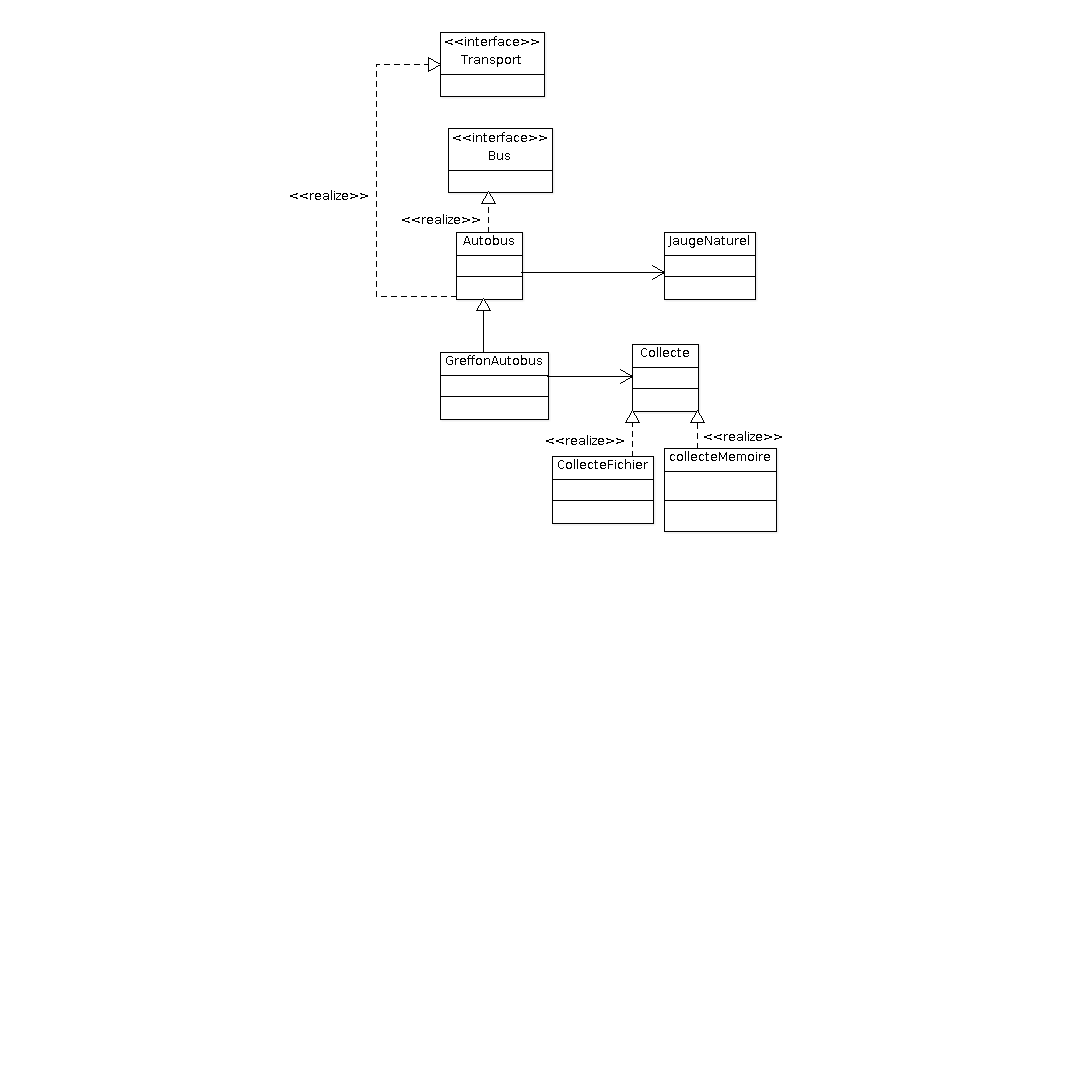
\includegraphics[scale=0.4]{est-un.png}

\end{figure}


\begin{figure}

    \caption{Diagramme de class EST-UN}
    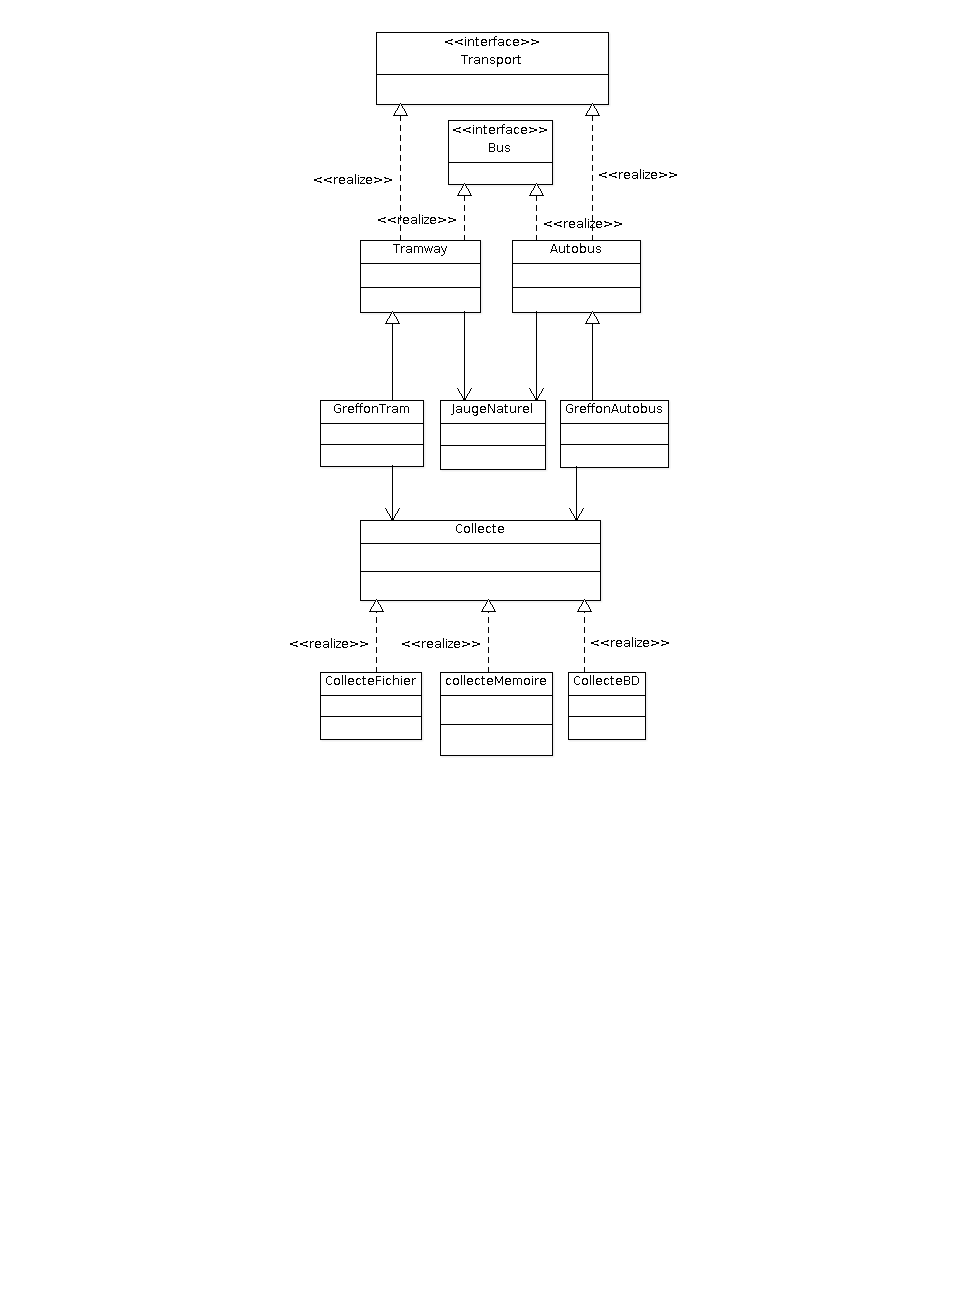
\includegraphics[scale=0.4]{est-un2.png}

\end{figure}


\section{Gestion d’erreurs et instanciation}

\subsection{Lever une exception}

\subsection{Capturer une exception}

\section{Paquetage tec}

\subsection{Utilisation des exceptions contrôlées et non-contrôlées}

\section{Remplacement d'un tableau par une collection}

\subsection{Java Collection Framework}


\subsection{Remaniement de la classe Autobus}
\subsubsection{Problème}

\subsection{Solutions}
\section{Commentaires}

\begin{itemize}
\item Pierre:
\item Victor:
\item Aurélien :
\item Lionel :
\item Reda :
\end{itemize}



\end{document}
